\documentclass[11pt]{article}
\usepackage[margin=1in]{geometry}
\usepackage{times}
\usepackage{microtype}
\usepackage{booktabs}
\usepackage{graphicx}
\usepackage{amsmath}
\usepackage[hidelinks]{hyperref}
\usepackage{caption}
\captionsetup{font=small,labelfont=bf}
\setlength{\parskip}{3pt}

\title{\textbf{Choose Again Each Loop:\\Expert Re-selection and the One-Loop Tax\\in a Small Looped Transformer}}
\author{David Ternoposkiy\\Independent researcher\\\small Draft, November 2026}
\date{}

\begin{document}
\maketitle

\begin{abstract}
Looped (latent-recurrent) language models apply one shared block several times per token. When that block contains mixture-of-experts layers, a design choice arises that non-looped models do not have: whether the router picks an expert once or again on every loop. We study this choice in a 26M-parameter looped nGPT, built on the Dory recipe and extended with four small experts in the recurrent block, trained on 1.2B tokens per model with three seeds. With per-token routing, re-selecting the expert on every loop gives higher multi-step arithmetic accuracy than fixing the first-loop choice (71.3\% vs.\ 59.7\%). It wins on each of the three seeds, at equal test loss. In an earlier two-seed cycle, top-1 re-selection on each loop also beat top-2 routing fixed for all loops (87.4/85.8\% vs.\ 81.8/78.4\%). We hypothesise that the benefit comes from \emph{sequential} composition: the loop lets a token apply a chain of experts, possibly the same one several times, instead of a fixed parallel mixture. We propose experiments to separate these effects. We also report a negative result for looping itself at this scale. A model with the same parameters trained only at one loop matches the looped model at three loops (test loss 1.710 vs.\ 1.708) at a third of the inference compute. The within-model gain from extra loops is almost entirely recovery of the \emph{one-loop tax} described by Ladhak et al.\ (2026). Training on the mean loss over all loop counts reduces this tax about 2.5-fold.
\end{abstract}

\section{Introduction}
Looped transformers spend more compute per token by applying a shared block repeatedly \cite{dehghani2019,saunshi2025,geiping2025,zhu2025}. NVIDIA's Dory1.0-4B \cite{dory} brings this to a post-trained 4B model with a 16-layer input block, a 40-layer shared recurrent block and a 16-layer output block, trained with loop counts sampled from $\{1,2,3,4\}$. The companion paper on Elastic Latent Recurrence (ELR) \cite{elr} adds mixture-of-experts models and proposes \emph{cross-loop route replay}: experts are routed on the first loop only and the same assignment is reused on later loops. This cuts mixed-depth update time by 11.7\% with no measurable change in a ten-task average at 30B-A3B scale.

Route replay treats the routing decision as fixed across loops. But a looped model with experts can also do something a non-looped mixture-of-experts cannot. Over $k$ loops, top-1 routing that is re-selected each time applies a \emph{sequence} of up to $k$ experts, $E_{a_k}\circ\cdots\circ E_{a_1}$, possibly including the same expert several times, at the per-pass cost of a single expert. A top-$m$ router that picks once instead applies the same parallel mixture on every pass. This report gives first evidence, at small scale, that the sequential option matters for multi-step arithmetic. It also documents what looping itself does and does not buy at this scale.

Contributions:
\begin{itemize}\setlength\itemsep{1pt}
\item \textbf{Expert re-selection.} Per-token re-selection on each loop vs.\ a first-loop choice gives 71.3\% vs.\ 59.7\% arithmetic accuracy over three seeds, winning on every seed at equal loss. Per-sequence top-1 re-selection beats a fixed top-2 router on two seeds.
\item \textbf{A hypothesis and an experimental design} for separating sequential composition, repeated use of one expert, and parallel top-$m$ activation (Section~\ref{sec:hyp}).
\item \textbf{The one-loop tax at small scale.} A three-seed comparison with non-looped controls matched in parameters and, separately, in inference compute. At 26M parameters, looping does not beat the parameter-matched model.
\item \textbf{Averaging over loop counts} reduces the tax about 2.5-fold, consistent with ELR's finding that mixing depths within an update helps.
\end{itemize}

\section{Setup}
\paragraph{Model.} Width 320, 8 heads, context 256, BPE vocabulary of 4{,}096. A 4-layer input block, a 10-layer shared centre and a 4-layer output block. nGPT layers \cite{ngpt} with unit-norm states and weights, SwiGLU MLPs (width 896), RoPE and a sigmoid output gate on attention, as in Dory. The loop follows Dory: $s_0=x$, $u_t=N(s_{t-1}+x)$, $s_t=N(F(u_t))$. The base model (\emph{Plain}) has 26.06M parameters.

\paragraph{Experts.} Four SwiGLU experts of width 120 in the centre (+0.6M parameters), with Gumbel-softmax routing during training (temperature 1 to 0.3), argmax at test, a Switch-style balance loss \cite{switch} and a penalty on routing uncertainty (both weighted 0.05). Routing is either per sequence (from the mean of the first 32 token states) or per token (from each token's state). The expert is chosen either once before the first loop or anew before each loop from the current state. A top-2 variant mixes two experts with softmax weights.

\paragraph{Other variants.} \emph{Run index}: per-loop channel weights $a_k, b_k$ and a bias $e_k$, so that $u_t=N(a_k s+b_k x+e_k)$, initialised to reproduce Dory. \emph{Between}: a 6-layer block between loops (34.9M parameters). \emph{Loop controller}: a small head that outputs a distribution over $k\in\{1..4\}$ per expert, trained on the expected loss with a baseline.

\paragraph{Controls.} \emph{No-loop, 10 layers}: Plain trained and evaluated at $k{=}1$ only (same 26.1M parameters, a third of the inference compute of Plain at $k{=}3$). \emph{No-loop, 30 layers}: 30 distinct centre layers in one pass (53.6M parameters), equal to Plain at $k{=}3$ in inference FLOPs.

\paragraph{Data.} The main cycle uses 3.34B tokens over seven sets, each sampled with equal probability per batch row: TinyStories, generated arithmetic (levels 2 and 5--9, from one operation to nested brackets and variable tracking), question answering (SQuAD, HotpotQA, Natural Questions, Simple Wikipedia), mixed-topic texts with embedded word problems, arithmetic explained in words, ``compose a problem'' tasks verified by evaluation, and Orca-Math 200k with the GSM8K train split. An earlier cycle used only the first three. We removed every training document sharing a 16-token span (24 for stories) with validation or test, and every word problem sharing an 8-word span with GSM8K test.

\paragraph{Training.} 73{,}180 steps at batch $64\times256$ (1.2B tokens per model): 24k steps at $k{=}1$; 24k steps with $k$ drawn uniformly from $\{1,2,3,4\}$ for the whole batch, with 10\% of batches forced to $k{=}1$; 6k steps with a per-token cycle of loop counts; then rounds in which half of each batch comes from one set. Gradients flow only through the final loop (TBPTL depth 1), as in Dory. AdamW, learning rate $6\cdot10^{-3}$, cosine decay, bf16, one RTX 4090 per model. The loop count is \emph{synchronized} across the batch, which is the schedule \cite{elr} identifies as paying the tax.

\paragraph{Evaluation.} Test cross-entropy on 512 windows of 256 tokens per set, averaged over sets. Arithmetic accuracy on 500 held-out problems by greedy decoding and exact match. Each configuration in the main cycle is trained on seeds 0, 1 and 2. Within a seed, all models share initial weights of common layers and the data order.

\section{Results}

\begin{figure}[t]
\centering
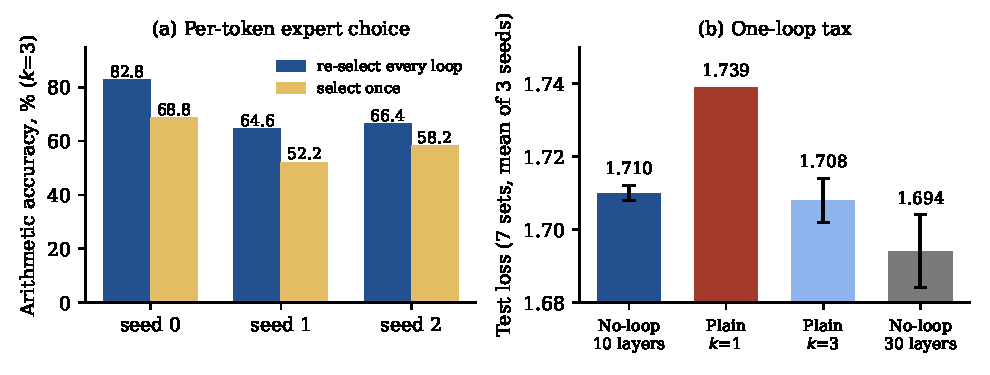
\includegraphics[width=\linewidth]{fig1.pdf}
\caption{(a) Arithmetic accuracy of the per-token expert model with run index: re-selecting the expert on each loop vs.\ fixing the first-loop choice. Test loss is 1.711 for both. (b) Mean test loss over three seeds; error bars are standard deviations where available. A parameter-matched model trained at one loop equals Plain at three loops.}
\label{fig:main}
\end{figure}

\subsection{Re-selecting the expert on each loop}
\paragraph{Per-token routing (three seeds).} We compare two otherwise identical per-token expert models with run index. One chooses each token's expert anew before every loop, the other once before the first loop. Test loss is identical (1.711), but arithmetic accuracy is 71.3\% vs.\ 59.7\%. Re-selection wins on every seed (82.8/64.6/66.4 vs.\ 68.8/52.2/58.2; Figure~\ref{fig:main}a). On seed 0 almost the whole gap lies in levels 6 and 7 (chains of 6--12 numbers), solved at 93\% and 77\% vs.\ 59\% and 43\%. Re-selection is not better than Plain (65.6\%, within noise), and the fixed choice is lower than Plain by an amount within the seed spread. The clearest statement is therefore relative: \emph{fixing the expert across loops hurts compared with re-selecting it}.

\paragraph{Per-sequence routing (earlier cycle, two seeds).} Table~\ref{tab:seq} compares per-sequence models on the three-set data. Top-1 routing re-selected on each loop gives the highest arithmetic accuracy in Table~\ref{tab:seq} on both seeds, ahead of a top-2 router fixed for all loops and of a top-1 router chosen once. Loss differences are within 0.01. Two caveats apply. These models had separate warm-ups. And on the seven-set data, per-sequence re-selection had the worst loss of all models (1.768 $\pm$ 0.035, Table~\ref{tab:main}), so the per-sequence result does not carry over to more diverse data. The per-token result does.

\begin{table}[t]
\centering\small
\begin{tabular}{lcc}
\toprule
Model (per-sequence routing, three-set data) & Test loss, $k{=}3$ & Arithmetic, $k{=}3$ (\%) \\
& seed 0 / 1 & seed 0 / 1 \\
\midrule
Top-1, re-selected each loop & 1.893 / 1.893 & \textbf{87.4 / 85.8} \\
Top-2, chosen once & 1.899 / 1.892 & 81.8 / 78.4 \\
Top-1, chosen once (no loop controller) & 1.903 / 1.895 & 81.8 / 77.4 \\
Plain (no experts) & 1.894 / 1.885 & 81.8 / 82.6 \\
\bottomrule
\end{tabular}
\caption{Earlier cycle. The first two rows also had a learned loop controller; all rows had separate warm-ups. Losses are not comparable with Table~\ref{tab:main}.}
\label{tab:seq}
\end{table}

\subsection{Looping does not beat a parameter-matched non-looped model}
Table~\ref{tab:main} and Figure~\ref{fig:main}b summarise the three-seed results. Plain improves from 1.739 at one loop to 1.708 at three. But the same architecture trained only at one loop reaches 1.710 $\pm$ 0.002 and matches Plain at three loops on arithmetic too (65.5\% vs.\ 65.6\%), with a third of the inference compute. The extra loops mostly recover what random-$k$ training cost at $k{=}1$. This is the one-loop tax of \cite{elr}. In their GPT-0.5B ablation, synchronized uniform sampling without one-loop overrides reaches 1.708 at one loop, against 1.685 for a non-recurrent baseline. Here the tax remains even though 10\% of batches are forced to $k{=}1$. These are whole batches, not ELR's within-step rank overrides, so each update still covers a single depth. Spending the same inference compute on distinct layers gives the best loss (1.694 $\pm$ 0.010), with twice the parameters. Run-index conditioning, per-token routing and the other variants differ from Plain by less than 0.01 in loss, within the seed spread.

\begin{table}[t]
\centering\small
\begin{tabular}{lrcc}
\toprule
Model & Params & Test loss & Arithmetic (\%) \\
\midrule
No-loop, 10 layers ($k{=}1$) & 26.1M & 1.710 $\pm$ 0.002 & 65.5 $\pm$ 7.3 \\
No-loop, 30 layers ($k{=}1$) & 53.6M & \textbf{1.694} $\pm$ 0.010 & 70.6 $\pm$ 4.8 \\
\midrule
Plain & 26.1M & 1.708 $\pm$ 0.006 & 65.6 $\pm$ 4.6 \\
Plain + run index & 26.1M & 1.708 $\pm$ 0.009 & 66.7 $\pm$ 5.6 \\
Plain + run index, no norm & 26.1M & 1.711 $\pm$ 0.004 & 69.3 $\pm$ 4.1 \\
Per-sequence experts, re-selected each loop & 26.6M & 1.768 $\pm$ 0.035 & 66.6 $\pm$ 10.6 \\
Per-token experts, re-selected each loop & 26.6M & 1.716 $\pm$ 0.005 & 69.9 $\pm$ 4.0 \\
Per-token experts + run index, re-selected each loop & 26.6M & 1.711 $\pm$ 0.013 & \textbf{71.3} $\pm$ 10.0 \\
Per-token experts + run index, chosen once & 26.6M & 1.711 $\pm$ 0.012 & 59.7 $\pm$ 8.4 \\
Between-loop block + run index & 34.9M & 1.752 $\pm$ 0.012 & 64.1 $\pm$ 9.5 \\
\bottomrule
\end{tabular}
\caption{Main cycle (seven test sets), mean $\pm$ standard deviation over three seeds. Looped models are evaluated at $k{=}3$; no-loop models at $k{=}1$. For reference, Plain at $k{=}1$ averages 1.739.}
\label{tab:main}
\end{table}

\subsection{Averaging the loss over loop counts reduces the tax}
In the earlier cycle, several expert models shared one warm-up and differed only in their last 19{,}200 steps. Table~\ref{tab:avg} compares a control with a variant trained on the mean of the losses at $k=1,2,3,4$ for each sequence. The gap between $k{=}1$ and $k{=}3$ shrinks from 0.037--0.043 to 0.014--0.018, about 2.5-fold, while the loss at $k{=}3$ stays the same or improves. This agrees with ELR's finding that mixing depths within each update lowers loss at every $k$. The pattern differs, though: in ELR's sampling comparison (their Table~3) the gain grows slightly with $k$, while here it is largest at $k{=}1$ (0.030--0.034, against 0.007--0.009 at $k{=}3$). There was no non-looped control in this cycle, so we cannot say whether averaging removes the tax entirely.

\begin{table}[t]
\centering\small
\begin{tabular}{llccccc}
\toprule
Seed & Last-stage objective & $k{=}1$ & $k{=}2$ & $k{=}3$ & $k{=}4$ & $k{=}1$ minus $k{=}3$ \\
\midrule
0 & Control (sampled $k$, no controller) & 1.940 & 1.905 & 1.903 & 1.905 & 0.037 \\
0 & Mean loss over $k=1..4$ & 1.910 & 1.896 & 1.896 & 1.896 & 0.014 \\
1 & Control (sampled $k$, no controller) & 1.938 & 1.897 & 1.895 & 1.896 & 0.043 \\
1 & Mean loss over $k=1..4$ & 1.904 & 1.886 & 1.886 & 1.886 & 0.018 \\
\bottomrule
\end{tabular}
\caption{Earlier cycle (three-set data). Expert models with a shared warm-up; only the last 19{,}200 steps differ.}
\label{tab:avg}
\end{table}

\subsection{Negative results}
\begin{itemize}\setlength\itemsep{1pt}
\item \textbf{Experts as such.} Routing specialises without labels (0.2--1.3 bits of mutual information between data set and expert, vs.\ 0.001 for shuffled labels), but expert models are about 0.5\% worse in loss than Plain, and only two or three of four experts are used. Per-token experts carry almost no topic information (0.01--0.08 bits), so what they specialise in is still an open question.
\item \textbf{Learned loop controller.} It recovers sensible per-set loop counts without labels, but no win over the best fixed $k$ held on a second seed. With per-token routing it cannot save compute, because a token must run as many loops as any later token that attends to it.
\item \textbf{Between-loop block and learned input fusion.} Both are worse in loss than the plain loop.
\end{itemize}

\section{Hypothesis: sequential expert chains vs.\ parallel activation}
\label{sec:hyp}
We conjecture that re-selection helps because a looped model with top-1 routing can build a \emph{chain} of experts, one per pass, adapted to each token. Compared with activating $m$ experts at once, this has three potential advantages:
\begin{enumerate}\setlength\itemsep{1pt}
\item \textbf{Composition over summation.} A top-$m$ router applies $\sum_i g_i E_i$ on every pass; re-selection applies $E_{a_k}\circ\cdots\circ E_{a_1}$, whose terms can depend on intermediate results. This could help multi-step tasks such as chained arithmetic, where the gap appeared.
\item \textbf{Repetition.} The same expert can be chosen on several loops, which amounts to applying one specialised transform repeatedly, in the spirit of iterating one step of an algorithm. A fixed top-$m$ router cannot express ``apply $E_a$ three times, then $E_b$''.
\item \textbf{Flexibility at constant cost.} Each pass costs one expert. The number of \emph{distinct} experts a token uses, from 1 to $k$, is decided per token by the router rather than fixed by $m$.
\end{enumerate}
These are hypotheses, and the data so far cannot separate them. We propose the following comparison, each on three or more seeds, with arithmetic accuracy broken down by level:
\begin{itemize}\setlength\itemsep{1pt}
\item top-1, re-selected each loop (the current best);
\item top-1, re-selected, but forbidden from repeating the previous loop's expert (tests repetition);
\item top-1, re-selected, but forced to repeat the first-loop choice (equivalent to route replay);
\item top-2 and top-$k$, chosen once (parallel activation at higher per-pass cost);
\item top-2, re-selected each loop;
\item a compute-matched variant: top-$m$ in a single pass vs.\ top-1 over $m$ loops.
\end{itemize}
We will also log the per-token expert sequences, to measure how often experts repeat, how many distinct experts a token uses, and whether these statistics differ between problem levels.

\section{Limitations}
The models are about 150 times smaller than Dory and see about 5{,}000 times fewer tokens, so none of these results need transfer to 4B or to FFN-MoE layers with many experts. The expert results use four small experts and a single arithmetic task. The three-seed comparison resolves a gap of about 10 points; the per-sequence comparison has two seeds and separate warm-ups. We use the synchronized schedule and a parameter-free, replace-style state update, the family of rules that ELR finds worst. We have not yet tested the ELR recipe itself. The 30-layer control matches inference FLOPs but not parameters. All work was done by one person. Code (316 tests) and per-seed results are at \url{https://github.com/Davidooff/Spidory}; training logs are available on request.

\begin{thebibliography}{99}\small
\bibitem{dory} M.~Fishman, S.~Sun, S.~Acharya, F.~Ladhak, B.~Chmiel, S.~Akle Serano, R.~Banner, B.~Ginsburg, K.~C.~Puvvada. Dory1.0-4B: A Looped Normalized-GPT. arXiv:2611.03998, 2026.
\bibitem{elr} F.~Ladhak, S.~Acharya, S.~Akle Serano, S.~Sun, B.~Ginsburg, K.~C.~Puvvada. One Model to Loop Them All: Elastic Latent Recurrence for Language Models. arXiv:2610.12582, 2026.
\bibitem{ngpt} I.~Loshchilov, C.-P.~Hsieh, S.~Sun, B.~Ginsburg. nGPT: Normalized Transformer with Representation Learning on the Hypersphere. ICLR, 2025.
\bibitem{dehghani2019} M.~Dehghani, S.~Gouws, O.~Vinyals, J.~Uszkoreit, {\L}.~Kaiser. Universal Transformers. ICLR, 2019.
\bibitem{saunshi2025} N.~Saunshi, N.~Dikkala, Z.~Li, S.~Kumar, S.~J.~Reddi. Reasoning with Latent Thoughts: On the Power of Looped Transformers. ICLR, 2025.
\bibitem{geiping2025} J.~Geiping et al. Scaling up Test-Time Compute with Latent Reasoning: A Recurrent Depth Approach. 2025.
\bibitem{zhu2025} R.-J.~Zhu et al. Scaling Latent Reasoning via Looped Language Models (Ouro). arXiv:2510.25741, 2025.
\bibitem{switch} W.~Fedus, B.~Zoph, N.~Shazeer. Switch Transformers. JMLR, 2022.
\end{thebibliography}
\end{document}
